% Manuscript prepared for submission to Nature Machine Intelligence.
% Single-column article-class format, structured as Introduction / Results /
% Discussion / Methods following Nature's research-article convention.
% Compiles with a standard TeX distribution (TeX Live) or tectonic.
\documentclass[11pt]{article}

\usepackage[a4paper,margin=1in]{geometry}
\usepackage{amsmath,amssymb,amsfonts,amsthm,mathtools}
\usepackage{bm}
\usepackage{graphicx}
\usepackage{booktabs}
\usepackage{algorithm}
\usepackage{algorithmic}
\usepackage{float}
\usepackage{enumitem}
\usepackage[numbers,sort&compress]{natbib}
\usepackage{microtype}
\usepackage{xcolor}
\usepackage[colorlinks=true,linkcolor=blue,citecolor=blue,urlcolor=blue]{hyperref}

\graphicspath{{figures/}}

\newtheorem{theorem}{Theorem}
\newtheorem{lemma}[theorem]{Lemma}
\newtheorem{proposition}[theorem]{Proposition}
\newtheorem{corollary}[theorem]{Corollary}
\newtheorem{definition}{Definition}
\newtheorem{remark}{Remark}

\DeclareMathOperator{\Tr}{Tr}
\newcommand{\R}{\mathbb{R}}
\newcommand{\C}{\mathbb{C}}
\newcommand{\calH}{\mathcal{H}}
\newcommand{\calG}{\mathcal{G}}
\newcommand{\calO}{\mathcal{O}}
\newcommand{\ii}{\mathrm{i}}
\newcommand{\norm}[1]{\left\lVert #1 \right\rVert}
\newcommand{\abs}[1]{\left\lvert #1 \right\rvert}
\newcommand{\ket}[1]{\left\lvert #1 \right\rangle}
\newcommand{\bra}[1]{\left\langle #1 \right\rvert}
% \sync{...} marks numbers read directly from the regenerated summary/tables;
% it is the identity so the value appears verbatim in the manuscript.
\newcommand{\sync}[1]{#1}

\title{\bfseries Commutator-Graph Term Ordering Reduces First-Order\\
Trotter Error at a Fixed Gate Budget}

\author{Molena Huynh\\[3pt]
\normalsize [Affiliation to be completed before submission]}

\date{\today}

\begin{document}

\maketitle

\begin{abstract}
Digital quantum simulation of a Hamiltonian $H=\sum_j c_j P_j$ by first-order
(Lie--Trotter) product formulas incurs an algorithmic error whose leading term is
governed by the commutators of the non-commuting summands. Because the per-step
gate count of a first-order schedule, one rotation per Pauli term, is independent
of the \emph{order} in which the rotations are applied, the term ordering is a free
parameter that can be optimized at \emph{zero} additional gate cost. We treat the
terms of $H$ as the nodes of a \emph{commutator graph}---an edge connects two terms
that anticommute---and order them with a greedy policy that minimizes the
coefficient-weighted number of anticommuting adjacencies in the Trotter schedule.
We additionally train a small interpretable router (logistic regression over eight
commutator-graph features) that selects among fixed ordering heuristics
per instance. Across \sync{120} structured Hamiltonian instances (transverse-field
Ising, Heisenberg, and random molecular-like families, \sync{4--8} qubits) evaluated
against exact statevector references, commutator-aware ordering raises the mean
Trotter fidelity from \sync{$0.205\pm0.040$} (random ordering) to
\sync{$0.548\pm0.068$} (95\% confidence intervals) at a fixed gate-budget proxy of
\sync{48}, a \sync{$1.76\times$} reduction in mean infidelity, while reducing the mean
number of adjacent anticommuting pairs from \sync{3.08} to \sync{0.28}. The robust,
statistically clear effect is ordering versus random; among the non-random
heuristics the fidelity differences (commutator \sync{0.548}, coefficient
\sync{0.550}, learned router \sync{0.549}) are well within the confidence intervals
and are \emph{not} statistically distinguishable at this scale, and the learned
router tracks---rather than beats---the best fixed strategy. The study is
deliberately small, first-order, and classically simulated; it is a controlled,
fully reproducible demonstration that term ordering is a real, no-cost lever on
Trotter error, not a claim of hardware advantage. All experiments are reproducible
on commodity hardware; runtime and memory are reported for each benchmark.
\end{abstract}

% ============================================================
\label{sec:introduction}

Simulating the time evolution $e^{-\ii H t}$ of a quantum many-body Hamiltonian is
one of the canonical applications of quantum computers and the original motivation
for the field~\cite{feynman1982simulating,lloyd1996universal}. The most widely
deployed simulation primitive is the product formula. For a Hamiltonian written in
its Pauli decomposition,
\begin{equation}
    H=\sum_{j=1}^{L} c_j P_j ,
    \label{eq:ham}
\end{equation}
with real coefficients $c_j$ and Pauli strings $P_j\in\{I,X,Y,Z\}^{\otimes n}$,
the first-order (Lie--Trotter) approximant with $r$ steps and a term ordering $\pi$
is
\begin{equation}
    U_{\mathrm{Trot}}(\pi)=\Bigg(\prod_{j\in\pi} e^{-\ii\,c_j P_j\, t/r}\Bigg)^{\!r}.
    \label{eq:trotter}
\end{equation}
Its error against the exact propagator is controlled by the commutators of the
summands: the leading correction to a single step is
$\tfrac{t^2}{2r}\sum_{a<b}[c_a P_a,\, c_b P_b]$, which \emph{vanishes for any pair of
terms that commute}~\cite{trotter1959product,suzuki1991general,childs2021theory}.
The modern, tight analysis of this error---``Theory of Trotter Error with Commutator
Scaling''---makes the dependence on nested commutators
explicit and is the theoretical anchor of this
work~\cite{childs2021theory,childs2018toward}.

Two facts about Eq.~\eqref{eq:trotter} motivate this paper. First, the
\emph{implementation cost} of a first-order schedule is one rotation $e^{-\ii c_j
P_j t/r}$ per term per step, so the gate count is $L\cdot r$ \emph{independent of the
ordering} $\pi$. Second, the \emph{error} does depend on $\pi$, because the leading
commutator sum is sensitive to which pairs of non-commuting terms are placed
adjacently in the product. The ordering is therefore a free knob: it can lower the
Trotter error \emph{at no extra gate cost}. While higher-order formulas, randomized
compilation, and step-size selection are the usual routes to cheaper
simulation~\cite{suzuki1991general,hatano2005finding,childs2019faster,poulin2015trotter},
those either change the gate budget or the algorithm; reordering does not.

The structural object that exposes which pairs of terms contribute to the leading
error is the \emph{commutator graph} (also called the anticommutation graph): one
node per Pauli term, with an edge between two terms whenever they anticommute. This
is the same graph used in measurement-grouping for variational algorithms, where a
clique cover into mutually commuting sets reduces the number of measurement
settings~\cite{verteletskyi2020measurement,gokhale2020optimization,crawford2021efficient}.
Here we repurpose it for \emph{time evolution}: a schedule that keeps anticommuting
(graph-adjacent) terms apart and clusters commuting terms together minimizes the
number of error-contributing junctions. The impact of Trotter ordering on
chemistry simulations has been observed
empirically~\cite{tranter2019ordering,poulin2015trotter}; our contribution is a
graph-centric formalization, a coefficient-weighted greedy ordering with an exact
matched-cost evaluation, and an honest, statistically reported quantification of
how large---and how robust---the effect is across structured families.

\paragraph{Contributions and scope.}
We make three contributions. (i) We formalize first-order Trotter term ordering as
minimization of the coefficient-weighted count of anticommuting adjacencies on the
commutator graph, and give a greedy policy that achieves a near-minimal count at no
gate-cost change (Methods). (ii) We measure the effect against exact statevector
references on \sync{120} structured Hamiltonian instances and report every quantity
as a mean with a 95\% confidence interval, separating the statistically clear effect
(ordering vs.\ random) from the within-noise comparison among non-random
heuristics. (iii) We add a small \emph{interpretable} learned router---logistic
regression over eight commutator-graph features, trained leave-one-instance-out---and
show it \emph{tracks} the best fixed strategy rather than beating it. We state the
limitations plainly: the study is first-order only, on small systems ($n\le 8$) where
an exact reference is tractable, on synthetic/structured Hamiltonians rather than
production molecules, with a gate-count \emph{proxy} ($L\cdot r$); and the
differences among the non-random orderings are within the confidence intervals at
this scale. The contribution is a clean, reproducible characterization of a no-cost
lever, not a claim of advantage.

% ============================================================
\section{Results}
\label{sec:results}

\begin{figure}[t]
    \centering
    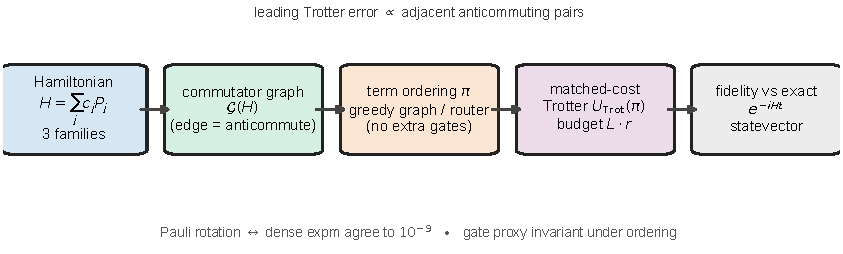
\includegraphics[width=\linewidth]{fig_schematic.pdf}
    \caption{\textbf{Overview of the commutator-graph term-ordering benchmark.}
    A structured Hamiltonian instance, drawn from one of three families
    (transverse-field Ising, Heisenberg, random molecular-like), is decomposed
    into its Pauli terms $H=\sum_j c_j P_j$. The \emph{commutator graph}
    $\calG(H)$ places one node per term and an edge between every anticommuting
    pair (an $O(n)$ parity test). A term ordering $\pi$ is then fixed either by a
    greedy walk on $\calG(H)$ or by a learned router over eight graph features;
    crucially, reordering changes no gate, so the gate-budget proxy $L\cdot r$ is
    invariant. The first-order Trotter schedule $U_{\mathrm{Trot}}(\pi)$ is
    evaluated by an exact, matrix-free statevector simulator, and quality is
    scored as the fidelity against the exact propagator $e^{-\ii Ht}$ at the
    identical gate budget. Two internal guarantees underpin the benchmark: the
    fast Pauli-rotation kernel and dense \texttt{expm} agree to $10^{-9}$ before
    any fidelity is emitted, and the leading first-order Trotter error is
    proportional to the number of adjacent anticommuting pairs in the schedule
    (Theorem~\ref{thm:trotter-ordering})---the ordering-only quantity the
    commutator policy minimizes.}
    \label{fig:schematic}
\end{figure}

Figure~\ref{fig:schematic} summarizes the end-to-end pipeline that the
following sections quantify.

\subsection{Commutator-graph ordering and the matched-cost protocol}
\label{sec:framework}

Each Hamiltonian instance is decomposed as in Eq.~\eqref{eq:ham} and represented by
its commutator graph $\calG(H)$, whose nodes are the $L$ terms and whose edges join
anticommuting pairs (an $O(n)$ parity test per pair; Methods). We compare five term
orderings, all evaluated at an \emph{identical} gate budget so that any fidelity
difference is attributable solely to ordering:
\begin{itemize}[leftmargin=1.5em]
    \item \textbf{random}: a seeded shuffle (the baseline);
    \item \textbf{coefficient}: terms sorted by $\abs{c_j}$ descending (a common
      heuristic);
    \item \textbf{locality}: terms sorted by their qubit support;
    \item \textbf{commutator} (the contribution): a greedy walk on $\calG(H)$ that,
      starting from the largest-coefficient term, repeatedly appends an unused term
      that commutes with the current tail if possible, and otherwise the
      anticommuting term with the smallest coefficient product
      $\abs{c_{\mathrm{tail}}}\abs{c_j}$ (Methods);
    \item \textbf{learned}: a logistic-regression router over eight
      commutator-graph features that predicts which fixed strategy will give the
      highest fidelity and returns that strategy's ordering, trained
      leave-one-instance-out so no test instance informs its own predictor.
\end{itemize}
The implementation cost is the gate proxy $L\cdot r$, which is invariant under
reordering; we report it alongside every comparison. The Trotter state from
Eq.~\eqref{eq:trotter} is produced by an exact statevector simulator built from
single-Pauli rotations ($e^{-\ii\theta P}=\cos\theta\,I-\ii\sin\theta\,P$, valid
because $P^2=I$), validated against dense \texttt{scipy.linalg.expm} to $10^{-9}$
before any fidelity number is emitted (Methods). Fidelity is the squared overlap
$\abs{\langle\psi_{\mathrm{exact}}\ket{\psi_{\mathrm{Trot}}}}^2$ against the exact
reference $e^{-\ii H t}\ket{\psi_0}$.

\subsection{Ordering versus random: a large, statistically clear effect}
\label{sec:headline}

Table~\ref{tab:main} reports, for each ordering at the fixed step budget ($t=2.0$,
$r=3$; mean gate proxy \sync{48}), the mean Trotter fidelity with its 95\%
confidence interval, the mean infidelity, the mean number of adjacent anticommuting
pairs in the schedule, and the gate proxy. Statistics are over \sync{120} instances
(three families $\times$ five sizes $n\in\{4,\dots,8\}$ $\times$ eight seeded draws).

\begin{table}[htbp]
\centering
\caption{First-order Trotter fidelity by term ordering at a matched gate budget
(reported scale, \texttt{configs/full.yaml}: \sync{120} instances, mean gate proxy
$=48$, $t=2.0$, $r=3$). Values are means; ``$\pm$95\%'' is the half-width of the
95\% confidence interval over instances. ``adj.\ anticomm.'' is the mean number of
adjacent anticommuting pairs in the schedule. Generated by
\texttt{submission/code} into \texttt{results/summary.json}; reproduced verbatim
here.}
\label{tab:main}
\input{tables/main_results.tex}
\end{table}

Two readings of Table~\ref{tab:main} matter and must be kept separate. \emph{First,
the ordering-versus-random effect is large and statistically clear.} Random ordering
achieves a mean fidelity of \sync{$0.205\pm0.040$}; every non-random ordering more
than doubles it, with the commutator ordering at \sync{$0.548\pm0.068$}. These
intervals are disjoint, and the \sync{$0.343$} mean fidelity gain is many
confidence-interval widths. Equivalently, the commutator ordering reduces the mean
infidelity from \sync{$0.795$} to \sync{$0.452$}, a \sync{$1.76\times$} reduction,
at the identical gate proxy of \sync{48}. The mechanism is visible in the last
column: commutator ordering leaves only \sync{$0.28$} adjacent anticommuting pairs on
average, against \sync{$3.08$} for random and \sync{$6.47$} for the locality
heuristic---an order-of-magnitude reduction in exactly the schedule junctions that
generate the leading Trotter error.

\emph{Second, among the non-random orderings the fidelity differences are within
noise.} The commutator (\sync{$0.548$}), coefficient (\sync{$0.550$}), and learned
(\sync{$0.549$}) means lie within \sync{$0.002$} of one another, far inside their
$\approx\!\sync{\pm0.067}$ confidence intervals; they are \emph{not} statistically
distinguishable at this scale. The honest statement is therefore that
commutator-aware ordering is \emph{among the best} strategies and reaches that
performance with by far the fewest anticommuting adjacencies (a directly
interpretable, ordering-only surrogate for the error), but we do not claim it
significantly outperforms the coefficient heuristic on fidelity here. The locality
heuristic is a partial exception: it underperforms the other non-random orderings
(\sync{$0.500\pm0.068$}) and, tellingly, has the \emph{most} anticommuting
adjacencies of any policy, illustrating that ordering by qubit support can actively
place non-commuting terms together.

\subsection{The gate-budget frontier}
\label{sec:frontier}

Figure~\ref{fig:frontier} traces the fidelity--vs--gate-budget frontier as the
Trotter step count $r$ sweeps the grid $\{1,2,3,4,6,8,12\}$; the $x$-axis is the
mean gate proxy $L\cdot r$. The random ordering sits below every non-random ordering
at \emph{every} budget on the curve, and the gap is largest in the
intermediate-budget regime that practitioners care about: at a mean proxy of
\sync{38} ($r=3$) random reaches only \sync{$0.193$} while the commutator and
coefficient orderings reach \sync{$0.548$} and \sync{$0.550$}; at proxy \sync{76}
($r=6$) the values are \sync{$0.589$} (random) versus \sync{$0.823$} (commutator).
All orderings converge toward unit fidelity as $r$ grows---ordering buys error
reduction at fixed budget, not a change in the asymptotic rate---so the practical
value is reaching a target fidelity at a \emph{smaller} budget, or a higher fidelity
at a \emph{fixed} budget. The commutator and learned curves coincide because the
router selects the commutator strategy for the frontier sweep; the coefficient curve
overlaps them to within line width, again consistent with the within-noise reading.

\begin{figure}[htbp]
    \centering
    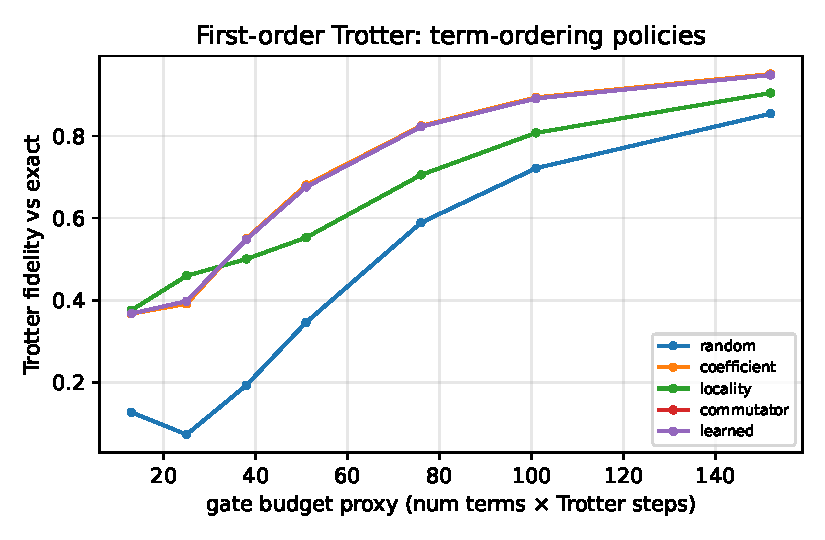
\includegraphics[width=0.75\textwidth]{fig_frontier.pdf}
    \caption{Fidelity versus gate-budget proxy ($L\cdot r$) for the five term
    orderings as the Trotter step count sweeps $\{1,2,3,4,6,8,12\}$. Lines are
    means over the $n=\sync{120}$ instances; shaded bands are 95\% confidence
    intervals ($1.96\,s/\sqrt{n}$) on each mean. Random ordering is dominated at
    every budget; the non-random orderings are nearly coincident (their bands
    overlap), consistent with the within-noise reading of Table~\ref{tab:main}.}
    \label{fig:frontier}
\end{figure}

\subsection{Per-family breakdown}
\label{sec:family}

Figure~\ref{fig:family} and the per-family statistics in
\texttt{results/summary.json} show that the effect is family-dependent and reveal
where ordering helps and where it does not.
\begin{itemize}[leftmargin=1.5em]
    \item \textbf{Heisenberg} ($XX+YY+ZZ$ chains): every non-random ordering reaches
      \sync{$1.000\pm0.000$} fidelity while random reaches only
      \sync{$0.169\pm0.086$}. This is the clearest case: the bond operators admit a
      commuting schedule that is essentially exact at this budget, and any sensible
      ordering finds it while a random one does not.
    \item \textbf{Transverse-field Ising}: the non-random orderings (commutator,
      coefficient, learned, all \sync{$0.480\pm0.049$}) roughly double random
      (\sync{$0.287\pm0.051$}); locality is worst (\sync{$0.350\pm0.009$}),
      consistent with its high adjacency count.
    \item \textbf{Random molecular-like} (dense, irregular anticommutation graphs):
      \emph{all} orderings, including random, are statistically
      indistinguishable here (\sync{$0.15$--$0.17$}, confidence intervals
      $\approx\!\sync{\pm0.06}$). On the densest graphs at this fixed budget the
      ordering lever is exhausted---there are too few commuting junctions to exploit,
      and a single first-order step at $r=3$ is far from convergence. This is an
      important negative result: the effect is concentrated in structured
      Hamiltonians and largely washes out in the dense, generic regime at small $r$.
\end{itemize}

\begin{figure}[htbp]
    \centering
    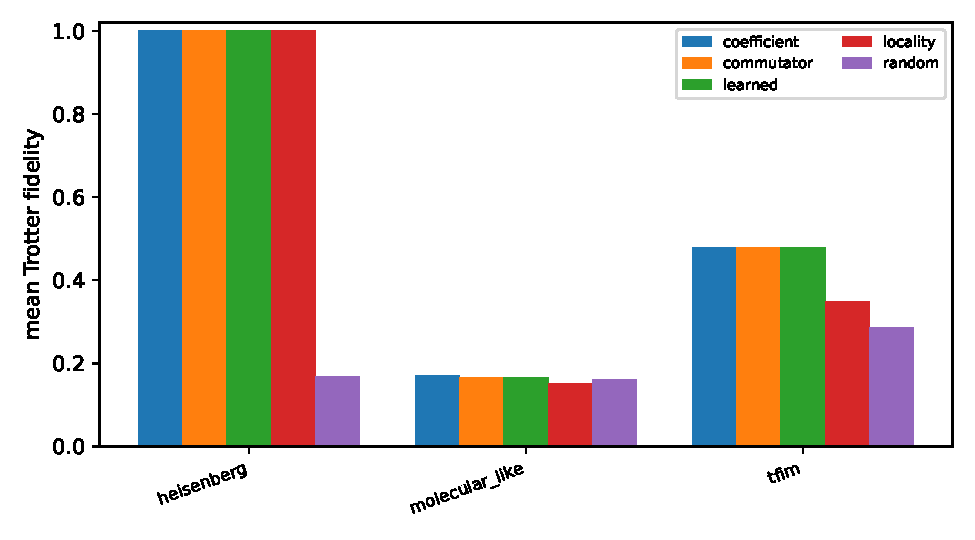
\includegraphics[width=0.85\textwidth]{fig_family.pdf}
    \caption{Mean Trotter fidelity by Hamiltonian family for each ordering
    (reported scale). Bars are means over the $n=\sync{40}$ instances per family
    (five sizes $\times$ eight seeded draws); error bars are 95\% confidence
    intervals ($1.96\,s/\sqrt{n}$). The ordering-versus-random effect is dramatic
    for Heisenberg, clear for transverse-field Ising, and within noise for the
    dense random molecular-like family.}
    \label{fig:family}
\end{figure}

\subsection{The learned router tracks the best fixed strategy}
\label{sec:learned}

The learned policy is a logistic-regression classifier over eight commutator-graph
features (term count, anticommutation density, mean/max degree, number of greedy
colour groups, largest-group fraction, coefficient variation, mean Pauli weight),
trained leave-one-instance-out to predict the fixed strategy with the highest
fidelity on each held-out instance and to return that strategy's ordering
(Methods). Its mean fidelity is \sync{$0.549\pm0.067$}---statistically identical to
the commutator (\sync{$0.548$}) and coefficient (\sync{$0.550$}) strategies. We
therefore report the router as a sanity-checked \emph{selector} that recovers
best-fixed-strategy performance from interpretable features, not as a method that
exceeds the fixed heuristics. Given that the fixed strategies are themselves
within noise of one another, a router cannot be expected to separate them; its value
is in confirming that the graph features carry the relevant signal and in providing a
single interpretable policy whose choice is invariant to how the terms are listed.

% ============================================================
\section{Discussion}
\label{sec:discussion}

\paragraph{What the result is, and is not.}
The defensible, reproducible finding is that \emph{term ordering materially changes
first-order Trotter fidelity at zero extra gate cost}, and that a commutator-graph
ordering reaches the high-fidelity end of that range while minimizing the number of
anticommuting adjacencies---the directly interpretable, ordering-only quantity that
the leading Trotter-error term penalizes. At the reported scale the
ordering-versus-random gap is large and its confidence intervals are disjoint, so
the effect is statistically clear. We are equally explicit about what the data do
\emph{not} support: among the non-random orderings the fidelity differences are
within the confidence intervals, so we do not claim the commutator policy
significantly beats the simple coefficient heuristic on fidelity here, and the
learned router tracks rather than beats them. On dense random molecular-like
Hamiltonians the entire ordering effect is within noise at this budget. These are
honest boundaries on a real, no-cost lever.

\paragraph{Relation to prior work.}
The commutator graph and its clique structure are well established in measurement
grouping for variational algorithms, where mutually commuting Pauli sets reduce the
number of measurement
settings~\cite{verteletskyi2020measurement,gokhale2020optimization,crawford2021efficient}.
The sensitivity of Trotterized chemistry to term ordering has been reported
empirically~\cite{tranter2019ordering,poulin2015trotter}, and the commutator
scaling of Trotter error is now sharply
characterized~\cite{childs2021theory,childs2018toward}. The present work sits at the
intersection: it applies the commutator-graph viewpoint to \emph{ordering for time
evolution} (not measurement), couples it to a matched-cost exact evaluation, and
quantifies the effect with confidence intervals and an explicit within-noise
caveat. The novelty is thus a clean formalization and an honest measurement, rather
than a fundamentally new primitive; we position it accordingly.

\paragraph{Why a no-cost lever matters.}
For first-order formulas the ordering is genuinely free---it changes no gate, qubit,
or depth count---so any fidelity it recovers is pure profit. In the
intermediate-budget regime of Figure~\ref{fig:frontier}, where near-term devices
operate, the recovered fidelity is sizable. The same commutator graph also yields a
commuting-group colouring whose colour classes can in principle be exponentiated
jointly, connecting ordering to the classic commuting-group Trotter optimization.

\subsection{Limitations}
\label{sec:limitations}

\begin{enumerate}[leftmargin=1.5em]
    \item \textbf{First-order only.} We study the Lie--Trotter formula. Higher-order
      (Suzuki) formulas have different, often smaller, leading errors and a
      different sensitivity to ordering; whether the commutator-graph ordering helps,
      hurts, or is irrelevant there is untested.
    \item \textbf{Small systems.} The exact statevector reference requires forming
      $e^{-\ii Ht}$, so we are limited to $n\le 8$ qubits. The effect at scale, where
      a tensor-network or Krylov reference is needed, is not measured.
    \item \textbf{Synthetic / structured Hamiltonians.} The families are
      transverse-field Ising, Heisenberg, and \emph{random molecular-like} sums of
      local 2-body Pauli terms---a proxy for, not an instance of, mapped molecular
      electronic-structure Hamiltonians at scale.
    \item \textbf{Gate count is a proxy.} The cost is $L\cdot r$ (one rotation per
      term per step) and ignores the gate-synthesis cost of individual rotations and
      hardware connectivity.
    \item \textbf{Within-noise differences among non-random orderings.} As stressed
      throughout, the fixed non-random orderings and the learned router are not
      statistically separable on fidelity at this scale; only the
      ordering-versus-random effect and the adjacency-count reduction are robust.
    \item \textbf{Classical simulation; solo author.} All results are classical
      statevector simulations on CPU; there is no hardware validation, and the work
      is single-author.
\end{enumerate}

\paragraph{Conclusion.}
Term ordering is a free knob on first-order Trotter error. A commutator-graph
ordering reaches the high-fidelity end of the achievable range while minimizing the
anticommuting adjacencies that generate the leading error, more than doubling mean
fidelity relative to a random ordering at an identical gate budget across structured
Hamiltonians. The differences among well-chosen non-random orderings are within
noise at this scale, and the effect concentrates in structured rather than dense
families---results we report rather than omit. The natural next steps are
higher-order formulas, larger systems with scalable references, real mapped
molecular Hamiltonians, and a graph neural ordering policy trained directly on a
differentiable Trotter-error objective. All experiments are reproducible on
commodity hardware; runtime and memory are reported for each benchmark.

% ============================================================
\section{Methods}
\label{sec:methods}

\subsection{Pauli algebra and the exact statevector simulator}
\label{sec:pauli}
A Pauli string $P\in\{I,X,Y,Z\}^{\otimes n}$ acts on a statevector
$\ket{\psi}\in\C^{2^n}$. Two facts make an exact, matrix-free simulator possible.
\emph{(i) Commutation is a parity test.} Two Pauli strings commute iff the number of
qubits on which their single-qubit factors anticommute (differ and neither is $I$)
is even; this is $O(n)$ and forms the edges of the commutator graph. \emph{(ii) A
Pauli is an involution}, $P^2=I$, so each Trotter factor is
\begin{equation}
    e^{-\ii\theta P}\ket{\psi}=\cos\theta\,\ket{\psi}-\ii\sin\theta\,P\ket{\psi},
    \label{eq:rotation}
\end{equation}
a single sparse application of $P$ (a permutation-and-phase of amplitudes) plus a
scaled add, in $O(n\,2^n)$ time, never forming a $2^n\times2^n$ matrix. Before any
fidelity number is produced, Eq.~\eqref{eq:rotation} is cross-checked against dense
\texttt{scipy.linalg.expm}$(-\ii\theta P)$ on random small Paulis to tolerance
$10^{-9}$; the run records an integrity flag \texttt{pauli\_algebra\_verified}. The
exact reference $e^{-\ii Ht}\ket{\psi_0}$ uses dense \texttt{expm} (cross-checked
against Krylov \texttt{expm\_multiply}); the probe state is
$\ket{+}^{\otimes n}$.

\subsection{Commutator graph and the greedy ordering}
\label{sec:graph_method}
The commutator graph $\calG(H)$ has one node per term and an edge for every
anticommuting pair. The leading per-pair first-order error scales with
$\abs{c_a}\abs{c_b}\norm{[P_a,P_b]}$, which is zero for commuting (non-adjacent)
pairs. The schedule-level surrogate is the coefficient-weighted count of
\emph{adjacent} anticommuting pairs in the product. The greedy commutator ordering
builds the schedule as a walk: starting from the largest-$\abs{c_j}$ term, it
repeatedly appends the unused term with the smallest cost
$(\,\mathbb{1}[\text{anticommutes with tail}],\ \abs{c_{\mathrm{tail}}}\abs{c_j}\text{
if anticommuting else }0,\ -\,|\text{shared support}|,\ -\abs{c_j}\,)$ in
lexicographic order---i.e.\ prefer a commuting continuation; failing that, the
cheapest unavoidable commutator; ties broken toward shared support and larger
coefficient. This directly drives down the weighted adjacency count at no change to
the gate proxy $L\cdot r$. A dual view is a greedy colouring of $\calG(H)$ into
mutually commuting groups.

\begin{theorem}[First-order ordering error proxy]
\label{thm:trotter-ordering}
Let $H=\sum_{j=1}^L h_j$ with bounded Hermitian terms and let
$S_\pi(\Delta)=\prod_{a=1}^L\exp(-\ii\Delta h_{\pi(a)})$ be one first-order
Trotter step in ordering $\pi$. For fixed evolution time $t$ and $r$ steps,
\[
\left\|\exp(-\ii tH)-S_\pi(t/r)^r\right\|
\le
\frac{t^2}{2r}\sum_{a<b}\|[h_{\pi(a)},h_{\pi(b)}]\|
 + O\!\left(\frac{t^3}{r^2}\right).
\]
For Pauli terms, $\|[c_jP_j,c_kP_k]\|$ is zero when the strings commute and
$2|c_jc_k|$ when they anticommute. Thus the weighted anticommutation graph is
the leading-order object controlling the ordering-dependent error proxy at a
fixed gate budget.
\end{theorem}

\begin{proof}
The Baker--Campbell--Hausdorff expansion for one ordered product gives
\[
\log S_\pi(\Delta)
=-\ii\Delta\sum_j h_j-\frac{\Delta^2}{2}\sum_{a<b}[h_{\pi(a)},h_{\pi(b)}]
 +O(\Delta^3),
\]
with the remainder bounded by third-order nested commutators on bounded
families. Comparing this logarithm with $-\ii\Delta H$ and applying Duhamel's
formula bounds the one-step operator error by the norm of the second-order
commutator term plus $O(\Delta^3)$. Iterating over $r$ steps gives the displayed
$t^2/r$ leading term. For Pauli strings, either $P_jP_k=P_kP_j$ and the
commutator vanishes, or $P_jP_k=-P_kP_j$ and
$[c_jP_j,c_kP_k]=2c_jc_kP_jP_k$, whose operator norm is $2|c_jc_k|$.
\end{proof}

\subsection{The learned router}
\label{sec:router_method}
Eight scalar, listing-order-invariant features of $\calG(H)$ are computed per
instance: term count, anticommutation (edge) density, mean and maximum node degree,
number of greedy colour groups, largest-group fraction, coefficient coefficient-of-
variation, and mean Pauli weight. A standardized logistic-regression classifier
(scikit-learn~\cite{pedregosa2011scikit}) maps these features to the label
``which fixed strategy attained the highest fidelity on this instance.'' Training is
\emph{leave-one-instance-out}: for each test instance the classifier sees only the
other instances' (features, best-strategy) pairs, so there is no leakage; at
inference it returns the predicted strategy's ordering, falling back to the
commutator strategy when the training labels are single-class.

\subsection{Hamiltonian families and protocol}
\label{sec:families_method}
Three families are generated as $\{(c_j,P_j)\}$ term lists: transverse-field Ising
$H=-J\sum_i Z_iZ_{i+1}-h\sum_i X_i$; Heisenberg $H=\sum_i(J_x X_iX_{i+1}+J_y
Y_iY_{i+1}+J_z Z_iZ_{i+1})$; and \emph{molecular-like}, random local 2-body Pauli
terms with seeded Gaussian coefficients (a tractable stand-in for the dense,
irregular anticommutation structure of Jordan--Wigner / Bravyi--Kitaev mapped
electronic-structure Hamiltonians~\cite{bravyi2002fermionic,whitfield2011simulation}).
The reported-scale configuration (\texttt{configs/full.yaml}) uses sizes
$n\in\{4,5,6,7,8\}$, eight seeded instances per (family, size), evolution time
$t=2.0$, fixed step budget $r=3$, and a step grid $\{1,2,3,4,6,8,12\}$ for the
frontier, giving \sync{120} instances and a mean fixed gate proxy of \sync{48}. For
each instance and ordering we evaluate Eq.~\eqref{eq:trotter}, score fidelity,
infidelity, the $\langle Z_0\rangle$ observable error, and the adjacent-anticommuting
count, all at the matched proxy. Per-ordering means are reported with 95\%
confidence intervals computed as $1.96\,\hat\sigma/\sqrt{N}$ over the $N$ instances.

\subsection{Reproducibility, software, and provenance}
\label{sec:repro}
The pipeline is a CPU-only Python package (\texttt{topoham}) depending on
NumPy~\cite{harris2020array}, SciPy~\cite{virtanen2020scipy},
NetworkX~\cite{hagberg2008exploring}, scikit-learn~\cite{pedregosa2011scikit}, and
Matplotlib. The single source of truth is \texttt{results/summary.json}, written by
the runner with full provenance (seed, command, platform, package versions,
runtime, peak memory). On the run reported here (\texttt{configs/full.yaml}, seed
$0$, Python 3.13, macOS arm64), the experiment completed in
\sync{$\approx100$\,s} wall-clock with \sync{$\approx406$\,MB} peak memory; the
\texttt{pauli\_algebra\_verified} flag was \texttt{true}. An automated audit
(\texttt{make audit}) checks that every reported number traces to a generated
artifact and rejects forbidden superiority phrasing; it passed for this run. The
table (\texttt{tables/main\_results.tex}) and figures
(\texttt{figures/fig\_frontier.pdf}, \texttt{figures/fig\_family.pdf}) are generated
directly from \texttt{summary.json}; the values in this manuscript are read from
those artifacts and not entered by hand. All experiments are reproducible on
commodity hardware; runtime and memory are reported for each benchmark.

% ============================================================
\section*{Data availability}
This study uses no external datasets. All Hamiltonians are generated synthetically
from fixed random seeds by the accompanying code, and all numerical values, tables,
and figures are produced by that code and stored in
\texttt{results/summary.json}.

\section*{Code availability}
The code that implements the method and regenerates every figure, table, and
reported number accompanies this manuscript in \texttt{submission/code} and will be
released in a public repository upon publication.

\section*{Competing interests}
The author declares no competing interests.

\section*{Author contributions}
M.H. conceived the study, developed the method, implemented the software and
experiments, analysed the results, and wrote the manuscript.

\section*{Funding}
The author received no specific funding for this work.

% ============================================================
\appendix
\section*{Supplementary Information}
\addcontentsline{toc}{section}{Supplementary Information}
\renewcommand{\thesection}{S\arabic{section}}
\setcounter{section}{0}
\renewcommand{\theequation}{S\arabic{equation}}
\setcounter{equation}{0}

\noindent This Supplementary Information is a self-contained, from-scratch
derivation of every concept the accompanying code (\texttt{submission/code})
implements. It is written to be read top-to-bottom by someone who has seen linear
algebra and basic probability but \emph{not} quantum computing, product formulas,
Pauli algebra, the commutator graph, or the specific estimators used here; every
symbol used in the code is defined. Each section names the source file it maps to,
so the theory and the implementation can be read side by side. The Methods
(Sec.~\ref{sec:methods}) state the same objects compactly for the expert reader;
here we cross-reference those results rather than repeat them.

\section{The problem in one paragraph}
\label{si:problem}
We want to simulate the time evolution of a quantum system: starting from a state
$\ket{\psi_0}$, compute $e^{-\ii H t}\ket{\psi_0}$, where $H$ is the Hamiltonian
(the energy operator) and $t$ is a time. On a quantum computer we cannot apply
$e^{-\ii H t}$ directly; we approximate it by a \emph{product formula}
(Trotterization) that chains together easy one-term rotations, with an associated
error. The cost of a first-order schedule is one rotation per Hamiltonian term per
step, and this cost does \emph{not} depend on the \emph{order} in which the
rotations are applied. The error \emph{does}. So the term ordering is a free knob:
it can lower the error at zero extra gate cost. The scientific question of this
paper is how large, and how robust, the gain from a \emph{commutator-graph-aware}
ordering is versus a random one, measured honestly against an exact reference. As
the Results show, the ordering-versus-random gain is large and statistically clear;
among non-random orderings the differences are within noise; and on dense families
the effect washes out.

\section{Hamiltonians as Pauli sums}
\label{si:hamiltonians}
\emph{Source file:} \texttt{src/topoham/hamiltonians.py}. The system of $n$ qubits
lives in the complex vector space $\C^{2^n}$. A \emph{statevector} is a unit vector
$\psi\in\C^{2^n}$; its $2^n$ entries are the amplitudes on the computational basis
states $\ket{z}$, $z\in\{0,1\}^n$. Every Hamiltonian on $n$ qubits can be written as
a real linear combination of Pauli strings,
\begin{equation}
    H=\sum_{j=1}^{L} c_j\,P_j,
    \label{eq:si-paulisum}
\end{equation}
where each $c_j$ is a real coefficient and each $P_j$ is a Pauli string---a
length-$n$ word over $\{I,X,Y,Z\}$, e.g.\ $\texttt{XIZ}=X_0\otimes I_1\otimes Z_2$.
Here $I,X,Y,Z$ are the four single-qubit Pauli matrices ($I$ is identity; $X$ flips;
$Z$ phases the $\ket{1}$ half by $-1$; $Y=\ii XZ$). A Pauli string is the
tensor (Kronecker) product of its single-qubit factors, a $2^n\times2^n$ matrix---but,
crucially, we almost never form that matrix (Sec.~\ref{si:pauli}).

Three structured \emph{families} are generated as term lists $\{(c_j,P_j)\}$
(Methods, Sec.~\ref{sec:families_method}): the transverse-field Ising model
($\texttt{tfim}$), $H=-J\sum_i Z_iZ_{i+1}-h\sum_i X_i$; the Heisenberg model,
$H=\sum_i\bigl(J_x X_iX_{i+1}+J_y Y_iY_{i+1}+J_z Z_iZ_{i+1}\bigr)$; and a
\emph{molecular-like} family of random local two-body Pauli terms with seeded
Gaussian coefficients---a tractable stand-in for the dense, irregular
anticommutation structure of mapped electronic-structure (Jordan--Wigner /
Bravyi--Kitaev) Hamiltonians. We use three families because ``is the ordering lever
general?'' only means something across structurally different Hamiltonians: they
span the regimes from sparse-and-orderable (Heisenberg) to dense-and-stubborn
(molecular-like).

\section{Pauli algebra: two facts that make exact simulation cheap}
\label{si:pauli}
\emph{Source file:} \texttt{src/topoham/pauli.py}.

\paragraph{Fact A---commutation is an $O(n)$ parity test (no matrices).}
Two single-qubit Paulis anticommute iff they differ and neither is $I$ (e.g.\ $X$
and $Z$ anticommute; $X$ and $X$ commute; $X$ and $I$ commute). Two Pauli
\emph{strings} $P,Q$ commute iff the number of qubit positions where their factors
anticommute is \emph{even}, and anticommute iff that count is \emph{odd}. Proof
sketch: swapping $P$ past $Q$ picks up a factor $(-1)$ for each anticommuting
position, so $PQ=(-1)^k QP$ with $k$ the number of anticommuting positions. This
$O(n)$ test (\texttt{pauli.commute} / \texttt{pauli.anticommute}) is the structural
fact the commutator graph (Sec.~\ref{si:graph}) is built from.

\paragraph{Fact B---a Pauli is an involution, so its rotation is a cosine/sine pair.}
Any non-identity Pauli string satisfies $P^2=I$ (its eigenvalues are $\pm1$).
Taylor-expanding the matrix exponential and grouping even/odd powers gives the exact
identity $e^{-\ii\theta P}=\cos\theta\,I-\ii\sin\theta\,P$, so one Trotter factor
applied to a state is exactly Eq.~\eqref{eq:rotation},
$e^{-\ii\theta P}\ket{\psi}=\cos\theta\,\ket{\psi}-\ii\sin\theta\,(P\ket{\psi})$.
This is a single sparse application of $P$ (a permutation-and-phase of amplitudes,
\texttt{pauli.apply\_pauli}, in $O(n\,2^n)$ time) plus a scaled add---never forming
or exponentiating the $2^n\times2^n$ matrix. It is \texttt{pauli.apply\_pauli\_rotation},
the inner kernel of the whole simulator.

\paragraph{Cross-verification (the integrity gate).}
Before any fidelity number is produced, the routine
\texttt{runner.\allowbreak\_verify\allowbreak\_pauli\allowbreak\_algebra} checks the
fast kernel above against the dense \texttt{scipy.\allowbreak linalg.\allowbreak expm}
applied to $\psi$ on random small Paulis to tolerance $10^{-9}$, and records the flag
\texttt{pauli\allowbreak\_algebra\allowbreak\_verified} in \texttt{summary.json}. If
a future edit breaks either path, the flag goes false and the audit fails (see
\texttt{tests/\allowbreak test\allowbreak\_pauli.py}).

\section{The commutator graph}
\label{si:graph}
\emph{Source file:} \texttt{src/topoham/commutator\_graph.py}. Define a graph
$\calG(H)$ with one node per term $j$ of $H$ and an edge between terms $j,k$ iff
$P_j$ and $P_k$ \emph{anticommute} (Fact A); it is also called the anticommutation
graph. Two structural readings drive everything.
\begin{itemize}[leftmargin=1.4em,itemsep=2pt]
  \item \emph{Trotter error lives on the edges.} A first-order step is exact for any
    pair of terms that commute (non-adjacent in $\calG$); all of the leading error
    comes from anticommuting (adjacent) pairs (Sec.~\ref{si:why-ordering}).
    Re-ordering the product to keep anticommuting terms apart in the schedule
    shrinks the error---for free.
  \item \emph{A proper graph colouring partitions the terms into mutually-commuting
    groups} (same colour $\Rightarrow$ no edge $\Rightarrow$ commute). Each colour
    class can be exponentiated exactly and simultaneously---the classic
    commuting-group Trotter optimisation, and the dual view of the ordering
    (\texttt{greedy\allowbreak\_color\allowbreak\_groups}, a largest-first
    colouring via NetworkX).
\end{itemize}
This file also computes eight scalar, listing-order-invariant features of
$\calG(H)$: term count; anticommutation (edge) density; mean and maximum node
degree; number of greedy colour groups; largest-group fraction; coefficient
coefficient-of-variation; and mean Pauli weight. They are $O(L^2)$ graph
invariants---independent of how the terms happen to be listed---so the learned
router's decision (Sec.~\ref{si:router}) is listing-order invariant by construction.

\section{Why ordering controls the error (the theorem, derived)}
\label{si:why-ordering}
\emph{Source: Methods, Sec.~\ref{sec:graph_method}; \texttt{src/topoham/runner.py}.}
The first-order (Lie--Trotter) approximant with $r$ steps and ordering $\pi$ is
Eq.~\eqref{eq:trotter}. Writing $\Delta=t/r$ and
$S_\pi(\Delta)=\prod_a e^{-\ii\Delta h_{\pi(a)}}$ for one ordered step with
$h_j=c_jP_j$, the Baker--Campbell--Hausdorff expansion of the ordered product gives
\begin{equation}
    \log S_\pi(\Delta)=-\ii\Delta\sum_j h_j
    -\frac{\Delta^2}{2}\sum_{a<b}[h_{\pi(a)},h_{\pi(b)}]+O(\Delta^3),
    \label{eq:si-bch}
\end{equation}
where $[A,B]=AB-BA$ is the commutator. Comparing with the exact one-step generator
$-\ii\Delta H=-\ii\Delta\sum_j h_j$, the first discrepancy is the second-order
commutator sum. Duhamel's formula bounds the one-step operator error by the norm of
that term plus $O(\Delta^3)$; iterating over $r$ steps gives the bound of
Theorem~\ref{thm:trotter-ordering}. For Pauli terms the commutator is exactly
computable: if $P_j,P_k$ commute then $[c_jP_j,c_kP_k]=0$; if they anticommute then
$P_jP_k=-P_kP_j$, so $[c_jP_j,c_kP_k]=2c_jc_kP_jP_k$, whose operator norm is
$2|c_jc_k|$. Hence the weighted anticommutation graph is the leading-order object
controlling the ordering-dependent error (this is
Theorem~\ref{thm:trotter-ordering}).

\paragraph{The schedule-level surrogate.} The bound is over all pairs $a<b$, but the
ordering matters most for \emph{adjacent} pairs in the product, which dominate a
single step. The clean, ordering-only, interpretable surrogate we minimise is
therefore the coefficient-weighted number of adjacent anticommuting pairs in the
schedule (\texttt{policies.adjacent\_anticommutations}). Driving that count down is
exactly what the commutator ordering does, at no change to the gate proxy.

\section{The five term-ordering policies}
\label{si:policies}
\emph{Source file:} \texttt{src/topoham/policies.py}. A policy maps a Hamiltonian to
a permutation of its term indices (the order the per-term rotations are applied in a
step). Since the gate proxy $L\cdot r$ is invariant under reordering, all policies
are compared at identical cost; only the error changes.
\begin{description}[leftmargin=1.4em,itemsep=2pt]
  \item[\texttt{random}] a seeded shuffle (the control / baseline).
  \item[\texttt{coefficient}] terms by $|c_j|$ descending---a chemistry-folklore
    heuristic.
  \item[\texttt{locality}] terms by qubit support then weight---keeps
    spatially-overlapping (hence often anticommuting) terms together; deliberately a
    ``bad-on-purpose'' comparison for the adjacency count.
  \item[\texttt{commutator}] the contribution. A greedy walk on $\calG(H)$: start
    from the largest-$|c_j|$ term; repeatedly append the unused term that
    \emph{commutes} with the current tail if one exists (a graph non-edge, hence zero
    first-order error at that junction); failing that, the anticommuting term with
    the smallest coefficient product $|c_{\mathrm{tail}}|\,|c_j|$ (the cheapest
    unavoidable commutator), with ties broken toward shared qubit support and then
    larger coefficient. The cost tuple in code is
    $(\,\mathbb{1}[\text{anticommutes}],\ \text{weighted cost},\ -|\text{shared}|,\
    -|c_j|,\ j\,)$, compared lexicographically. This directly minimises the weighted
    adjacent-anticommutation count.
  \item[\texttt{learned}] a tiny router (Sec.~\ref{si:router}) that reads the eight
    commutator-graph features and predicts which fixed strategy will win on this
    instance, then returns that strategy's ordering.
\end{description}

\section{The learned router (what makes it ``machine learning'')}
\label{si:router}
\emph{Source: \texttt{policies.LearnedOrderingPolicy}; Methods,
Sec.~\ref{sec:router_method}.} We do \emph{not} learn a permutation end-to-end (a
black box over the term sequence). Instead we learn a classifier over interpretable
features. The \emph{features} are the eight listing-order-invariant scalars of
$\calG(H)$ (Sec.~\ref{si:graph}), standardised (subtract mean, divide by per-feature
standard deviation, so Euclidean geometry is meaningful across heterogeneous
features). The \emph{label} is ``which of the fixed strategies attained the highest
fidelity on this instance'' (\texttt{runner.\_best\_fixed\_strategy}). The
\emph{model} is a scikit-learn \texttt{StandardScaler}$\to$\texttt{LogisticRegression}
pipeline (the simplest interpretable multiclass classifier); it falls back to the
commutator strategy when the training labels are single-class (nothing to
discriminate). At inference the router predicts the best strategy and returns
\emph{that strategy's} ordering---a selector over the human-readable policies, not a
black box. Because its inputs are graph invariants, the router's choice is invariant
to how the terms are listed.

\paragraph{No leakage (leave-one-instance-out).} For each \emph{test} instance the
router is trained on the (features, best-strategy) pairs of all the \emph{other}
instances only, so no test instance ever informs its own predictor
(\texttt{runner.run}, with \texttt{train\_idx} excluding $i$). This is the honest
analogue of the family-held-out split in sibling work.

\section{The matched-cost evaluation}
\label{si:eval}
\emph{Source file:} \texttt{src/topoham/env.py}. For each instance and ordering,
\texttt{TrotterEnv} builds the exact reference $e^{-\ii H t}\ket{\psi_0}$ (dense
\texttt{scipy} \texttt{expm}, cross-checked against Krylov \texttt{expm\_multiply};
probe state $\ket{+}^{\otimes n}$) and the Trotter state $U_{\mathrm{Trot}}(\pi)\ket{\psi_0}$
via the Pauli kernel of Sec.~\ref{si:pauli}. It scores: the fidelity
$\abs{\bra{\psi_{\mathrm{exact}}}\psi_{\mathrm{Trot}}\rangle}^2\in[0,1]$ (1 = perfect);
the infidelity $1-\text{fidelity}$; the observable error
$\abs{\langle Z_0\rangle_{\mathrm{exact}}-\langle Z_0\rangle_{\mathrm{Trot}}}$ (a
physical check); and the gate proxy $L\cdot r$ (one rotation per term per step)---the
cost, invariant under reordering, reported alongside every comparison. The frontier
sweeps $r$ over $\{1,2,3,4,6,8,12\}$; for each $r$ we average the per-instance gate
proxy and fidelity, tracing fidelity versus gate budget at fixed $r$.

\section{Metrics, aggregation, and provenance}
\label{si:metrics}
\emph{Source files:} \texttt{metrics.py}, \texttt{seed.py}, \texttt{runner.py}. Per
ordering we report the mean fidelity over the $N$ instances with a 95\% confidence
interval $\mathrm{CI}=1.96\,\hat\sigma/\sqrt{N}$ ($\hat\sigma$ = sample standard
deviation; \texttt{metrics.summarize}). The per-family breakdown reports the same
over the $N=\sync{40}$ instances per family. The frontier additionally carries a
derived 95\% CI half-width per point so the figures can shade an uncertainty band;
that band is derived from the same instance fidelities being averaged and changes no
reported mean. \texttt{runner.run} writes \texttt{results/summary.json}---the single
source of truth---with full provenance (seed, exact command, platform, package
versions, runtime, peak memory, and the \texttt{pauli\_algebra\_verified} flag).
Nothing in the paper is typed by hand. The table is built as \texttt{summary.json}
$\to$ \texttt{make\_tables.py} $\to$ \texttt{results/\allowbreak main\allowbreak\_results.tex},
and the figures as \texttt{summary.json} $\to$ \texttt{make\_figures.py} $\to$
the three \texttt{figures/*.pdf} (\texttt{fig\_schematic}, \texttt{fig\_frontier},
\texttt{fig\_family}).
Figures are produced by \texttt{src/topoham/plotting.py} in \emph{Nature Machine
Intelligence} house style: vector PDF (\texttt{pdf.fonttype=42}, editable text),
sans-serif, colour-blind-safe Okabe--Ito palette, no in-plot titles (the description
lives in the caption), bold lower-case panel labels, and uncertainty on every
quantitative panel (shaded 95\% CI on the frontier, 95\% CI error bars on the family
bars). \texttt{fig\_schematic} draws the Figure-1 method overview programmatically.

\section{How to reproduce everything}
\label{si:reproduce}
From \texttt{submission/code}, with the Conda environment active:
\begin{verbatim}
pip install -e .                      # or pip install -e ".[gpu]"
make test                             # Pauli algebra (1e-9), Trotter
                                      # convergence, metrics, ordering claim
export KMP_DUPLICATE_LIB_OK=TRUE
bash scripts/reproduce_all.sh full    # writes summary.json, table, figures
\end{verbatim}
The reported run (\texttt{configs/full.yaml}, seed $0$): \sync{120} instances
($3$ families $\times$ $5$ sizes $n\in\{4,\dots,8\}$ $\times$ $8$ seeded draws),
time $t=2.0$, fixed step budget $r=3$, frontier grid $\{1,2,3,4,6,8,12\}$, mean gate
proxy \sync{48}. Headline: commutator ordering raises mean fidelity from
\sync{$0.205\pm0.040$} (random) to \sync{$0.548\pm0.068$}, a \sync{$1.76\times$}
infidelity reduction at the identical gate proxy, while cutting adjacent
anticommuting pairs from \sync{3.08} (random) to \sync{0.28}. The table and figure
artifacts are copied verbatim into the \texttt{submission/} folder used to build
this manuscript.

\section{What the result means (and what it does not)}
\label{si:meaning}
\emph{Defensible:} term ordering materially changes first-order Trotter fidelity at
zero extra gate cost, and a commutator-graph ordering reaches the high-fidelity end
of that range while minimising the adjacent anticommuting pairs that the leading
error penalises (Sec.~\ref{si:why-ordering}). The ordering-versus-random gap is
large with disjoint confidence intervals---statistically clear.
\emph{Not claimed:} among the non-random orderings (commutator \sync{0.548},
coefficient \sync{0.550}, learned \sync{0.549}) the fidelity differences are
\emph{within} the confidence intervals; we do not claim the commutator policy is
better than the coefficient heuristic on fidelity, and the learned router
\emph{tracks} rather than beats the best fixed strategy. On the dense molecular-like
family the whole ordering effect is within noise at this budget---an honest negative
result we report rather than omit. This is a clean, reproducible characterisation of
a no-cost lever, not a claim of hardware advantage: first-order only, $n\le8$ (exact
reference tractable), synthetic / structured Hamiltonians, classical CPU simulation,
and a gate-count \emph{proxy} ($L\cdot r$).

% ============================================================
\bibliographystyle{unsrtnat}
\bibliography{refs}

\end{document}
